\documentclass{beamer}
\usefonttheme[onlymath]{serif}

\usepackage[utf8]{inputenc}
\usepackage[T1]{fontenc}
\usepackage{lmodern}
\usepackage[francais]{babel}

% For table
\usepackage{booktabs} % To thicken table lines
\usepackage{multirow}
\usepackage{amsmath,amssymb,amsfonts}

\graphicspath{{img/}}

\usepackage{graphicx}
\usepackage{textcomp}
\usepackage{xcolor}
\usepackage[group-separator={,}]{siunitx}
\def\BibTeX{{\rm B\kern-.05em{\sc i\kern-.025em b}\kern-.08em
		T\kern-.1667em\lower.7ex\hbox{E}\kern-.125emX}}

\usepackage{booktabs} %top/mid/bottom rule

\definecolor{red}{RGB}{255,0,0}
\definecolor{green}{RGB}{0, 102, 0}
\definecolor{maron}{RGB}{102,51,0}
\definecolor{orange}{RGB}{255,128,0}
\definecolor{blue}{RGB}{0,153,153}

%for footnote
\usepackage{perpage} %the perpage package
\MakePerPage{footnote} %the perpage package command

\newcommand{\marouane}[1]{\textcolor{blue}{(#1 - MY)}}
\newcommand{\david}[1]{\textcolor{green}{(#1 - DG)}}

\usepackage{fontawesome}
\newcommand{\link}[2]{\href{#1}{#2~{\smaller\faExternalLink*}}}

\mode<presentation> {
	\usetheme{ulaval}
	\setbeamercovered{invisible}
}

\logo{
	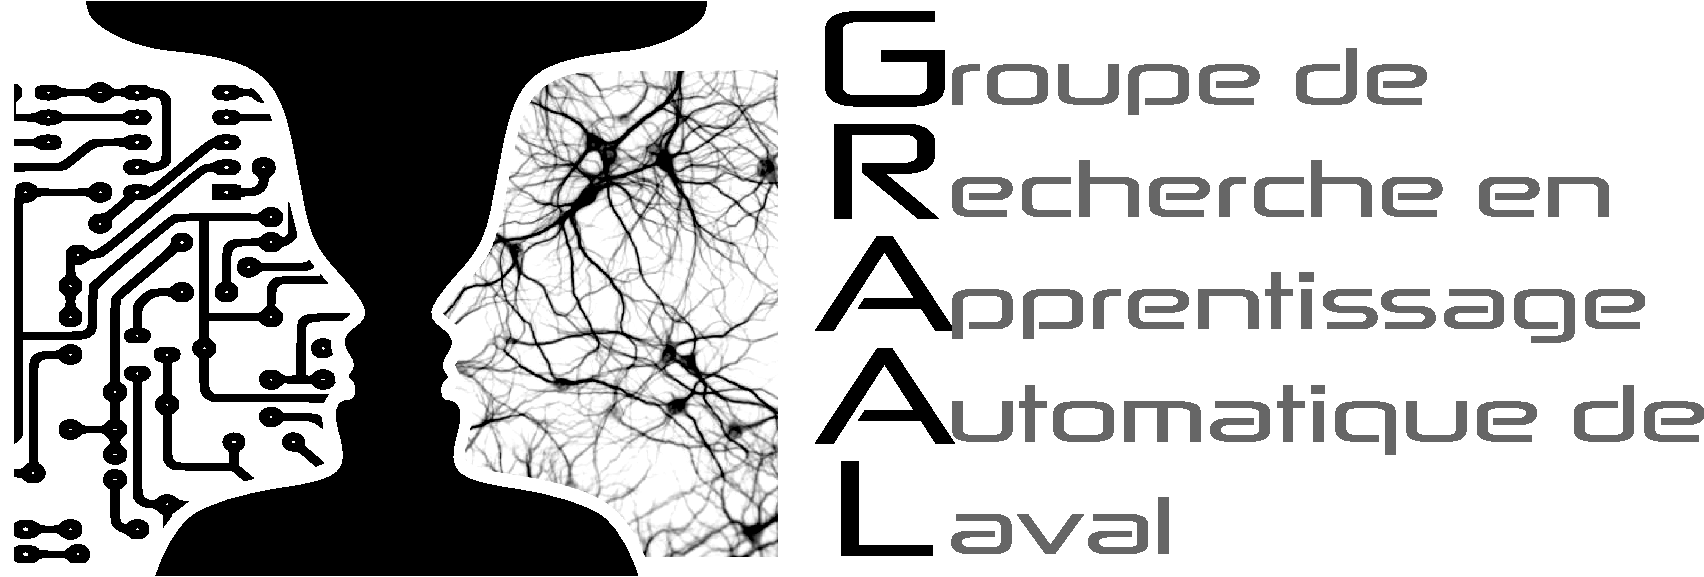
\includegraphics[height=0.65cm, keepaspectratio]{graal.pdf}\hspace{.2cm}\vspace{.85\paperheight}}


\title[Deepparse]{Deepparse et l'utilisation des sous-mots pour l'analyse syntaxique d'adresses multinationales}

\author[Yassine et al.]{David Beauchemin, M. Sc.}
\institute[Université Laval]
{
	{\emph{david.beauchemin@ift.ulaval.ca}}
}
\date{30 mai 2023}

\AtBeginSection[]
{
	\begin{frame}<beamer>
		\frametitle{Agenda}
		\tableofcontents[currentsection]
	\end{frame}
}

\begin{document}
	
	\begin{frame}[label=titre, plain]
		\titlepage
		\begin{center}
			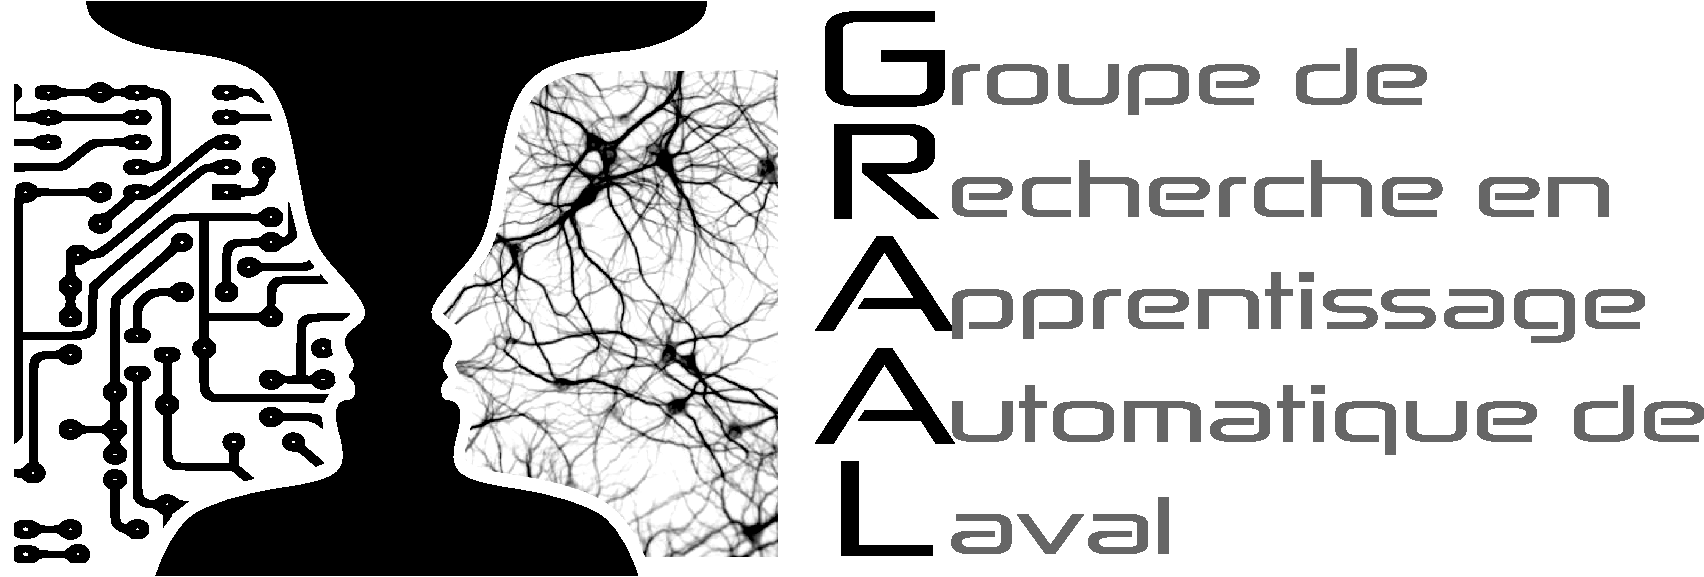
\includegraphics[height=1cm]{graal}
			
\includegraphics[height=1cm]{UL_P}
		\end{center}
	\end{frame}
	
	\begin{frame}{Votre conférencier}
		\begin{minipage}{0.25\linewidth}
			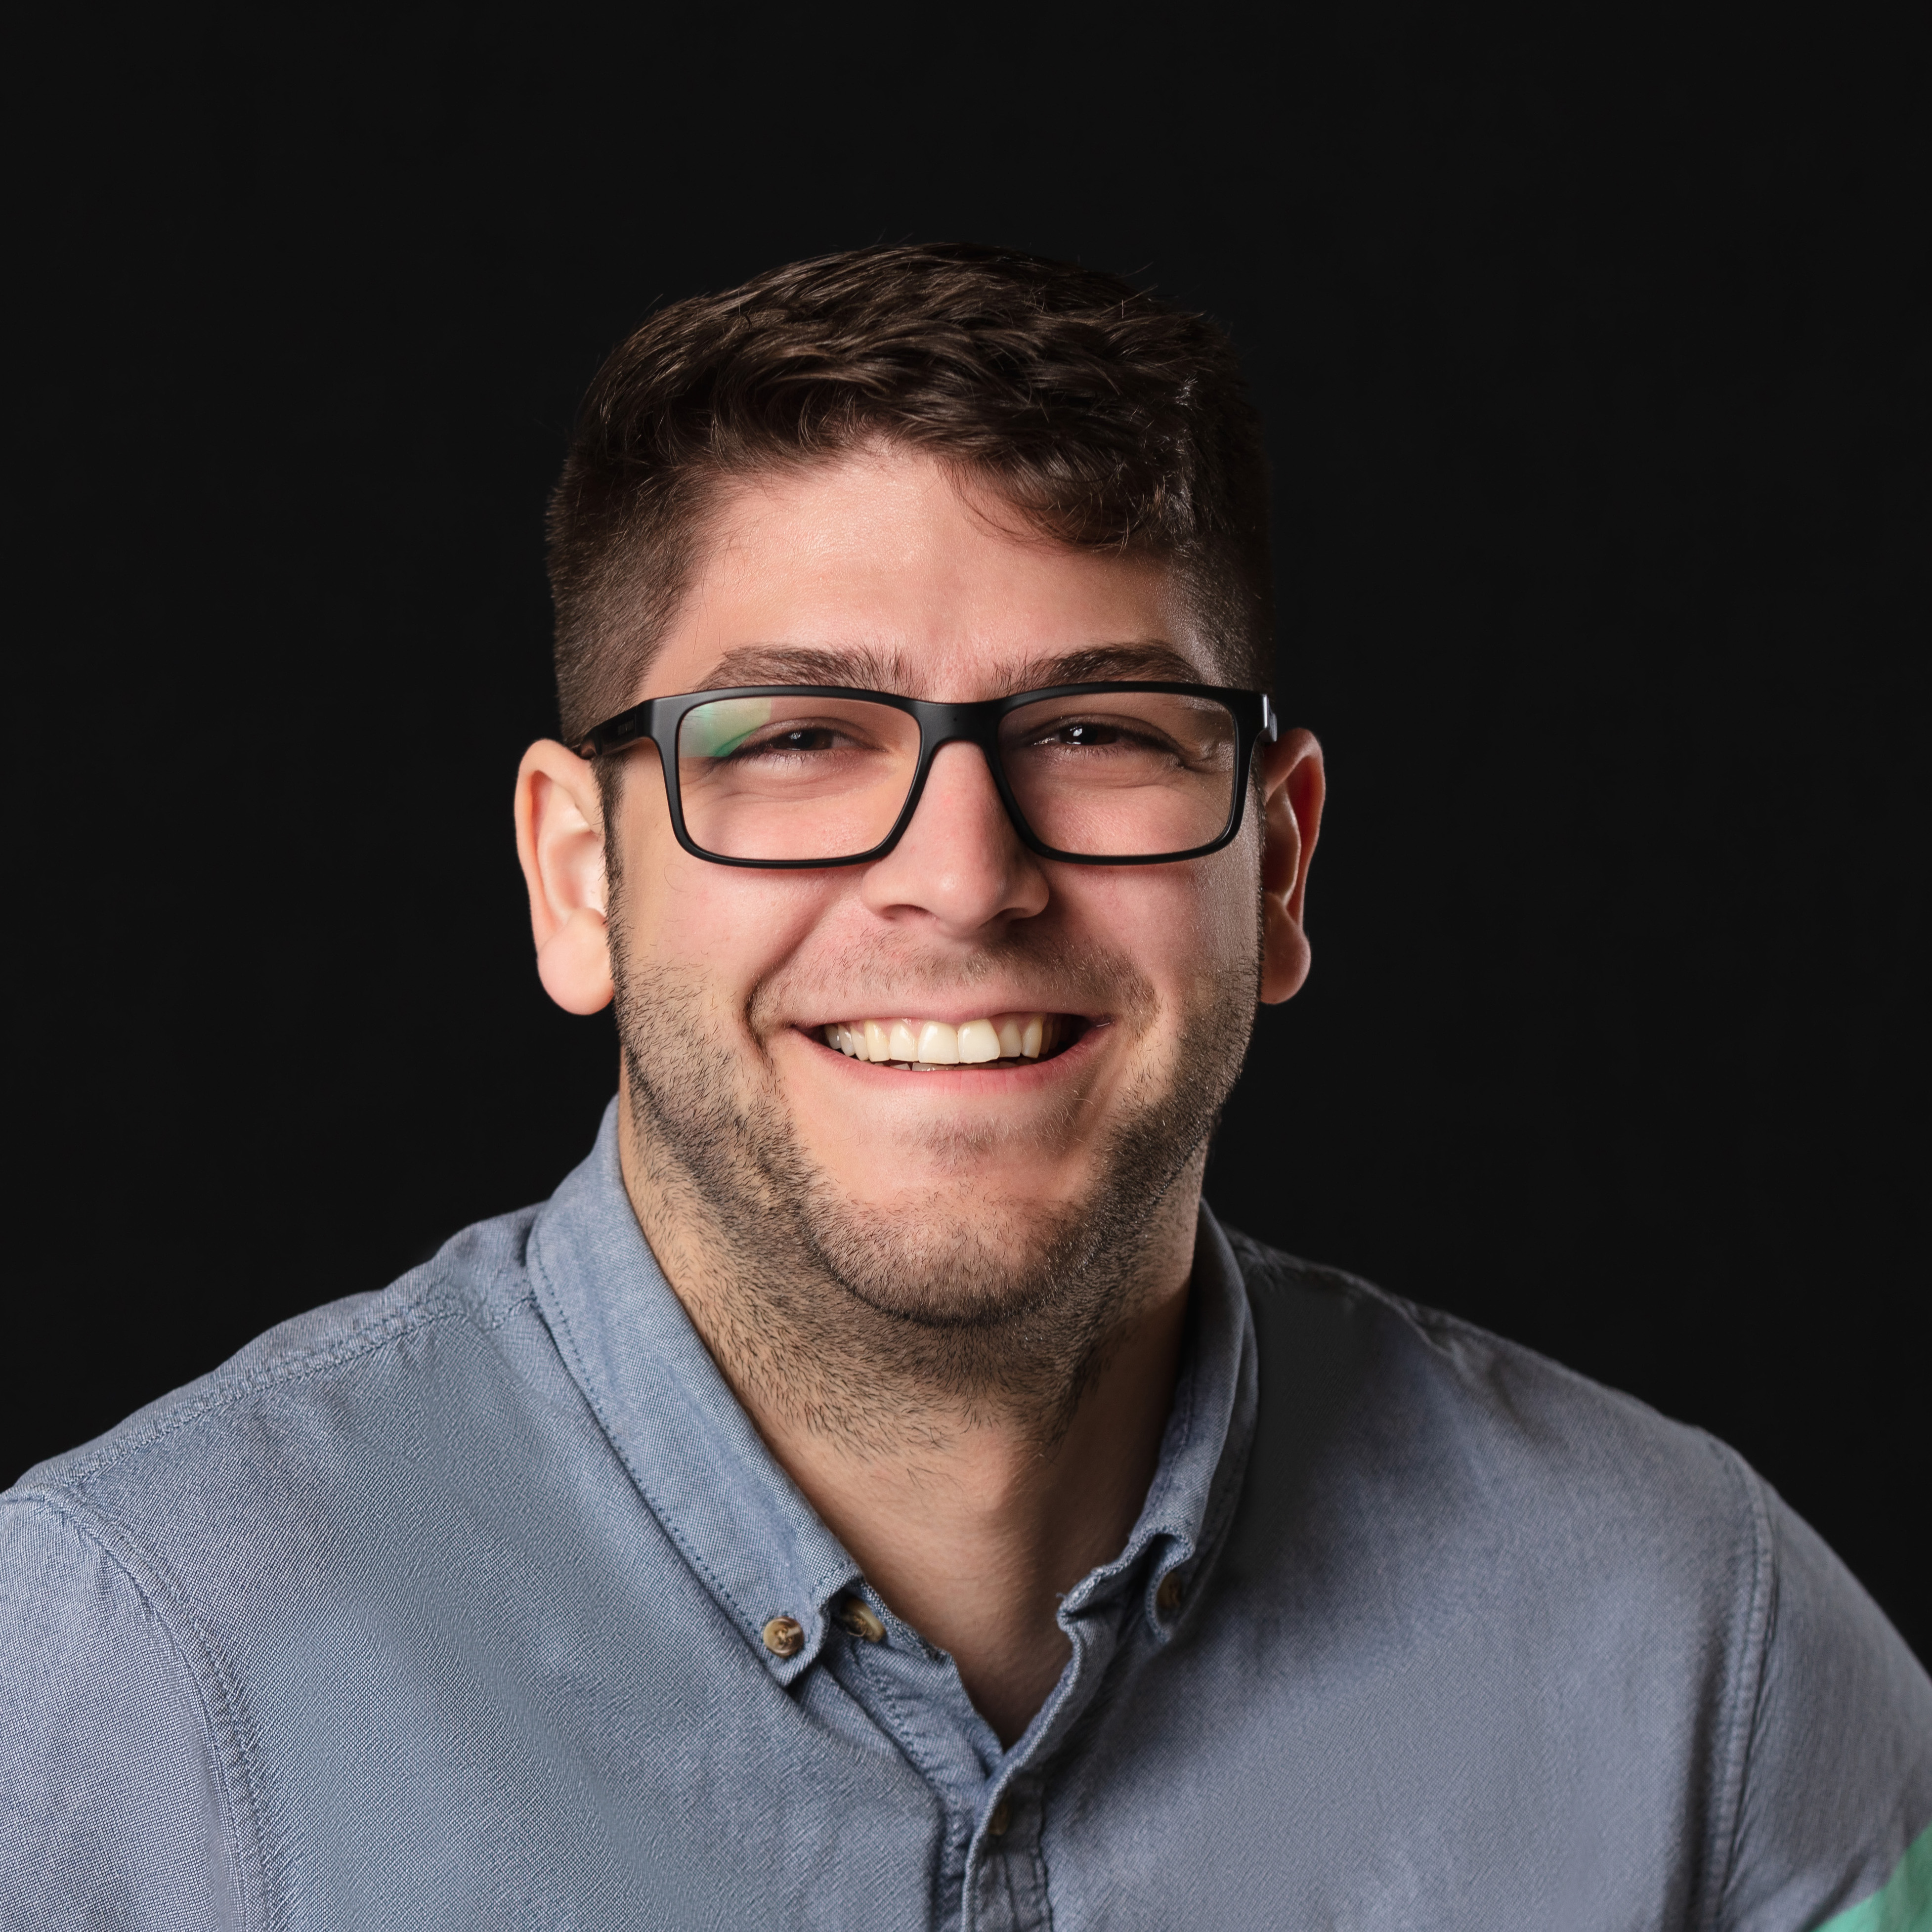
\includegraphics[width=\linewidth,keepaspectratio]{img/david}
		\end{minipage}
		\hfill
		\begin{minipage}{0.70\linewidth}
			\begin{itemize}
				\item B. Sc. en actuariat
				\item M. Sc. en informatique
				\item Candidat au doctorat en informatique
				\item Membre fondateur de la \link{https://baseline.quebec/}{coopérative de solidarité Baseline en intelligence artificielle}
				\item Fondateur et créateur d'\link{https://anchor.fm/open-layer}{OpenLayer}, un podcast bilingue sur l'IA
			\end{itemize}
		\end{minipage}
		
		\begin{minipage}{0.25\linewidth}
			\tiny\textbf{DAVID BEAUCHEMIN} \\
			Directeur général et candidat au doctorat en informatique
		\end{minipage}
	\end{frame}
	
	\begin{frame}{Objectifs de la conférence}
		\begin{itemize}
			\item Comprendre Deepparse.
			\item Connaitre les cas d'application de Deepparse.
			\item Connaitre comment Deepparse fonctionne (technique).
		\end{itemize}
	\end{frame}
	
	\section{Introduction}
	
	\begin{frame}{Introduction}
		Qu'est-ce que l'analyse d'adresses?
		\begin{figure}
			\centering
			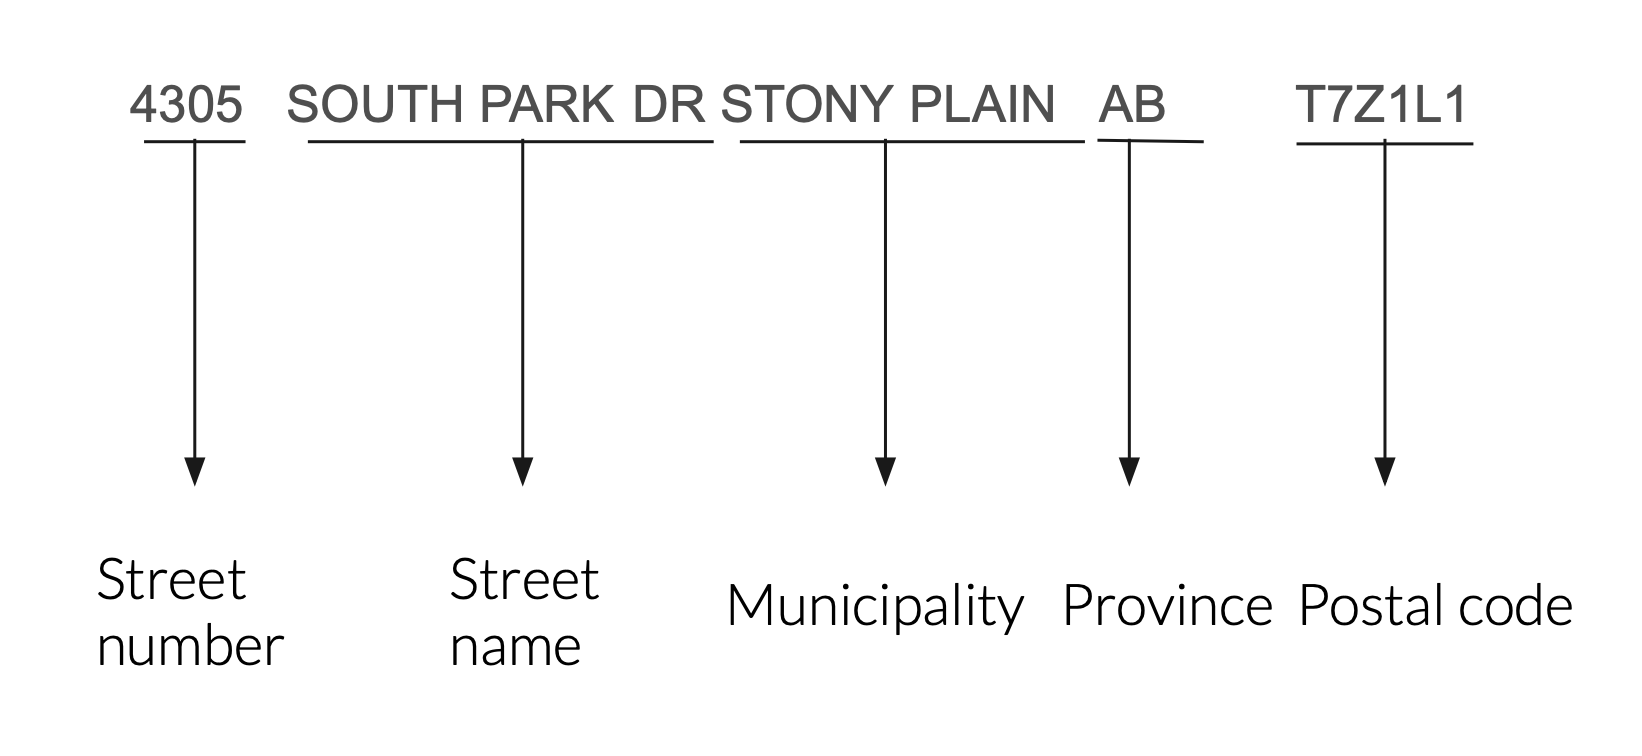
\includegraphics[width=\linewidth]{address_parsing_example.png}
		\end{figure}
		
		Utile pour des tâches telles que \textit{Record Linkage} et \textit{Geocoding}.
	\end{frame}
	
	\begin{frame}{Introduction}
		\begin{figure}
			\centering
			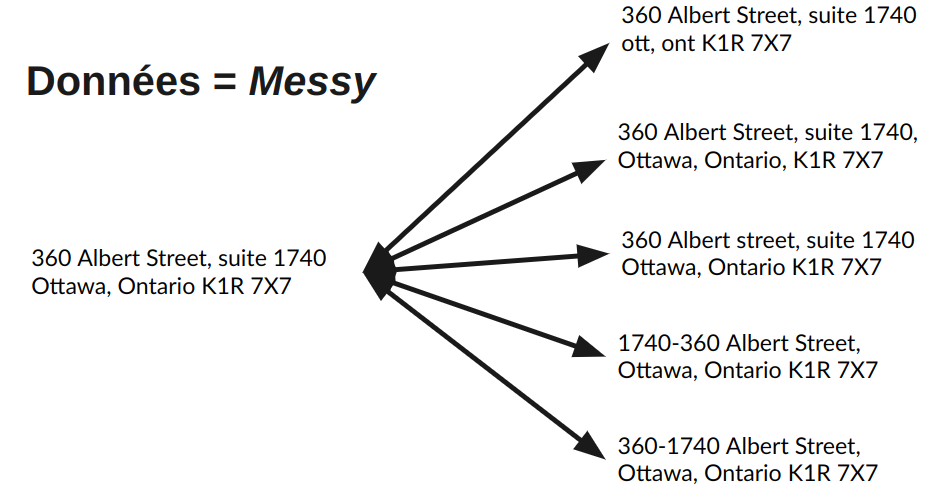
\includegraphics[width=0.7\linewidth]{img/messy}
		\end{figure}
	\end{frame}
	
	%	\section{Autres méthodes}
	%	\begin{frame}{Analyse des adresses}
		%		\begin{itemize}
			%			\item Méthodes basées sur des règles
			%			\item Modèles probabilistes
			%			\item Méthodes neuronales
			%		\end{itemize}
		%	\end{frame}
	%
	%	\begin{frame}{Libpostal}
		%		\begin{itemize}
			%			\item<1-> Modèle probabiliste
			%			\item<2-> Pré-traitement et post-traitement
			%			\item<3-> 1 milliard de données d'entraînement
			%		\end{itemize}
		%	\end{frame}
	
	\section{Deepparse}
	
	\begin{frame}{Deepparse}
		\begin{figure}
			\centering
			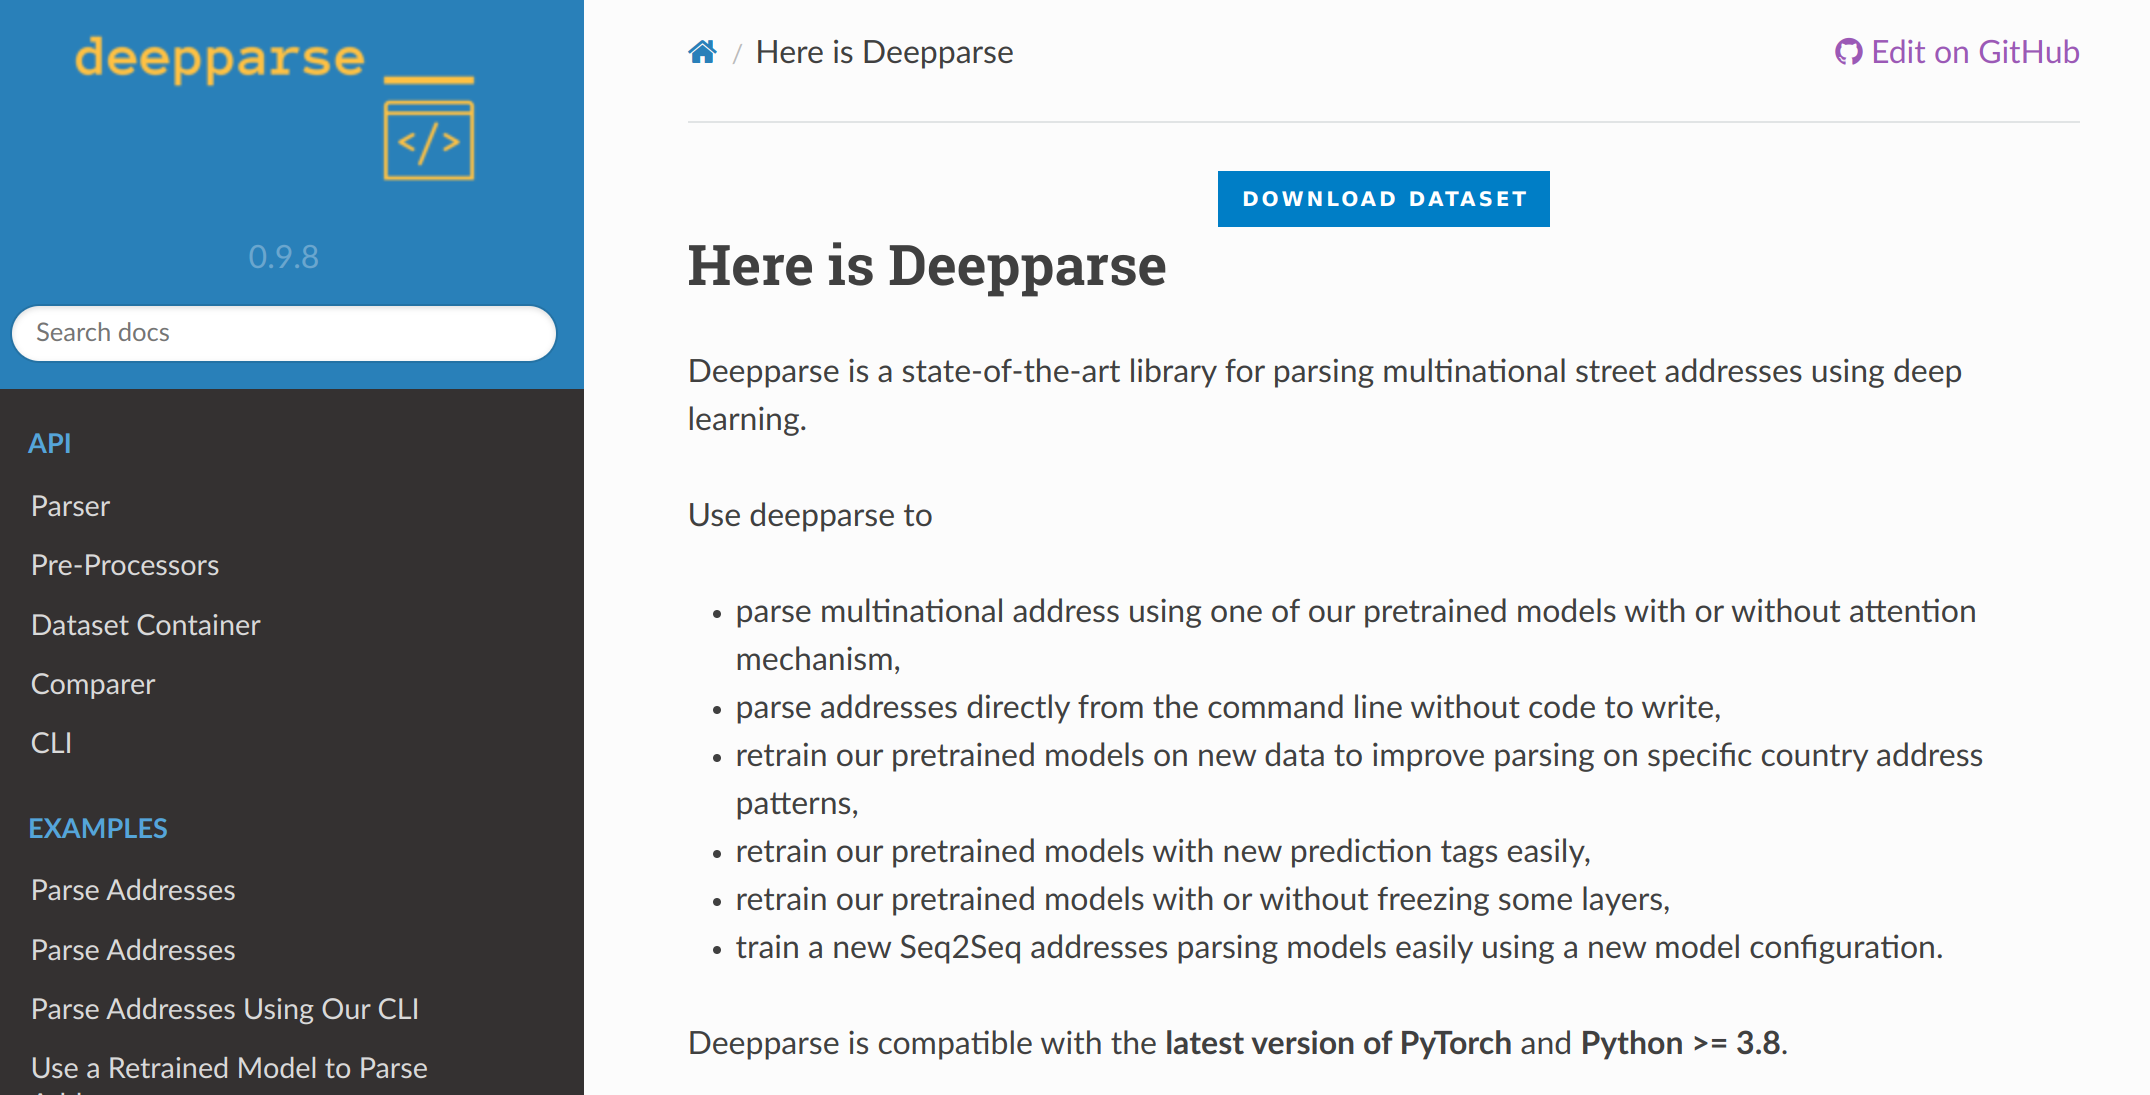
\includegraphics[width=\linewidth]{img/deepparse}
			\caption{\href{https://deepparse.org/index.html}{Documentation}}
		\end{figure}
	\end{frame}
	
	\begin{frame}{Particularités}
		\begin{figure}
			\centering
			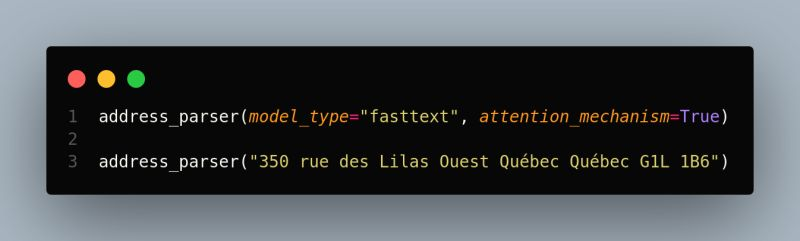
\includegraphics[width=0.7\linewidth]{img/parsing_python1}
		\end{figure}
		\begin{figure}
			\centering
			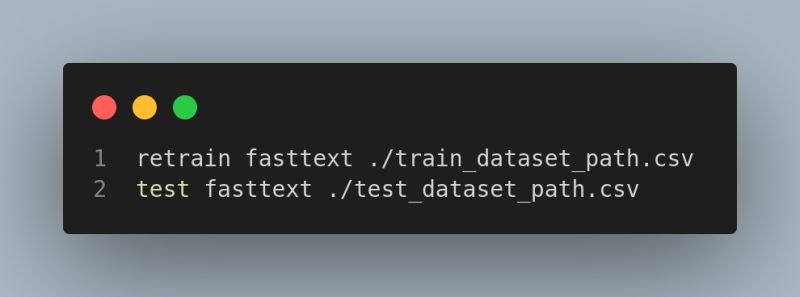
\includegraphics[width=0.7\linewidth]{img/parsing_python}
		\end{figure}
		\note{En Python, en ligne de commande ou sur un service infonuagique.}
	\end{frame}
	
	\begin{frame}{Particularités}
		\begin{figure}
			\centering
			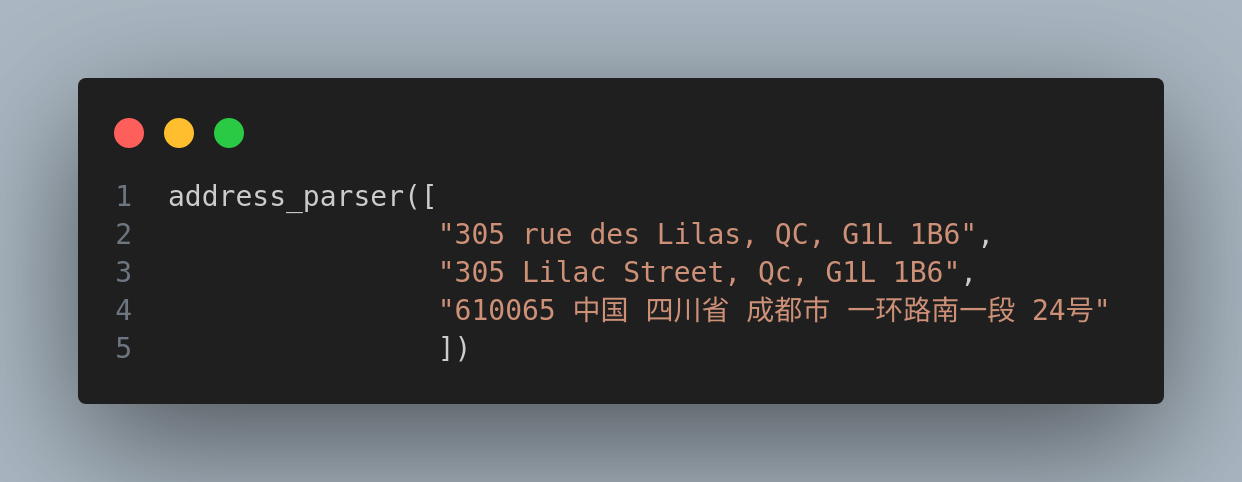
\includegraphics[width=0.7\linewidth]{img/multiseg}
		\end{figure}
		\note{Segmentation d'adresses internationales avec un seul modèle.}
	\end{frame}
	
	\begin{frame}{Particularités}
		\begin{figure}
			\centering
			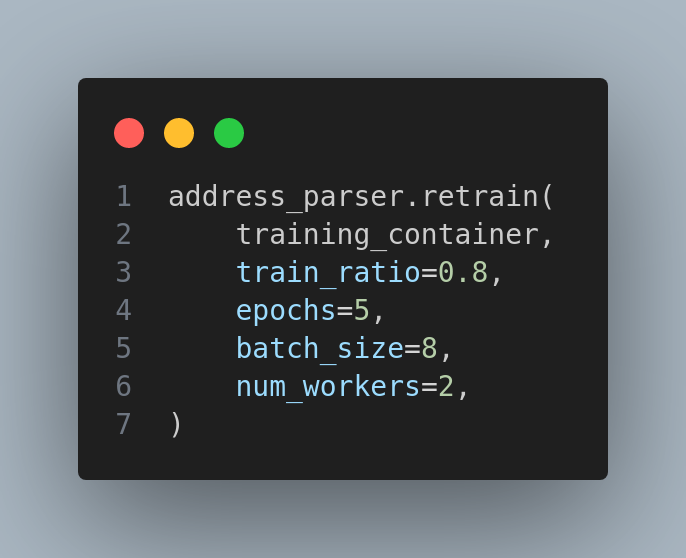
\includegraphics[width=0.6\linewidth]{img/retrain}
		\end{figure}
		\note{Ajustement des modèles de bases sur de nouvelles données.}
	\end{frame}
	
	\begin{frame}{Particularités}
		\begin{figure}
			\centering
			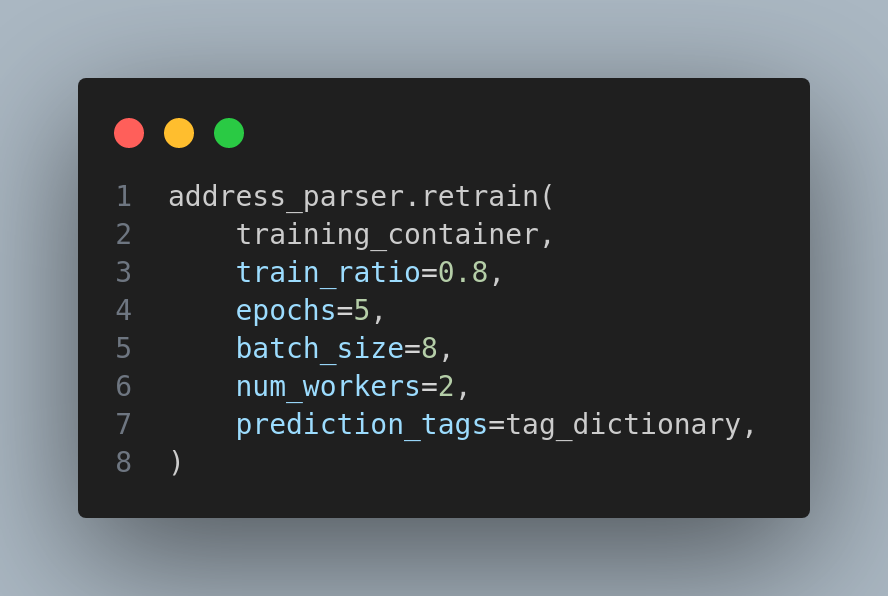
\includegraphics[width=0.6\linewidth]{img/new_tags}
		\end{figure}
		\note{Ajustement des modèles sur de nouvelles étiquettes.}
	\end{frame}
	
	\begin{frame}{Particularités}
		\begin{figure}
			\centering
			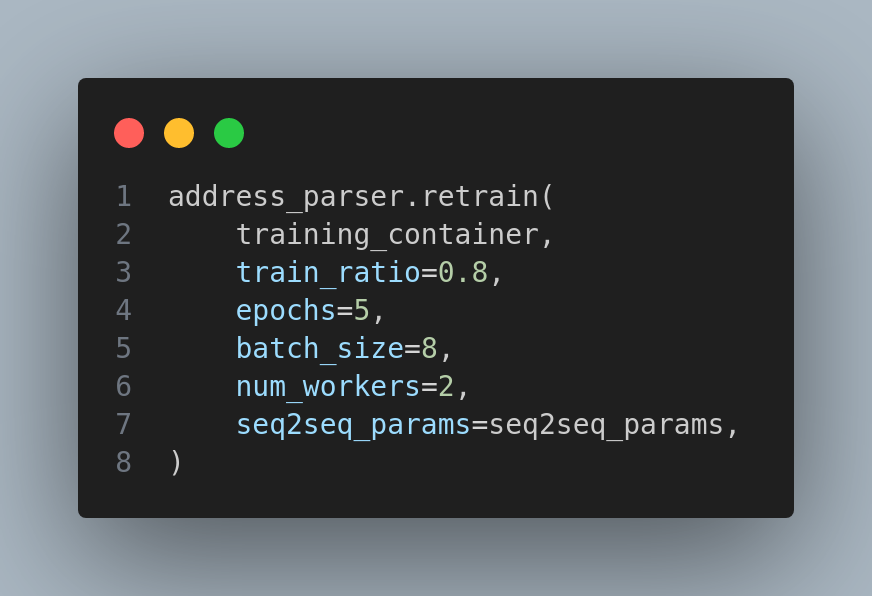
\includegraphics[width=0.7\linewidth]{img/new_archi}
		\end{figure}
		\note{Modification de l'architecture pour besoin spécifique.}
	\end{frame}
	
	\section{Cas d'utilisation}
	\begin{frame}{Similarité d'entité}
		\begin{figure}
			\centering
			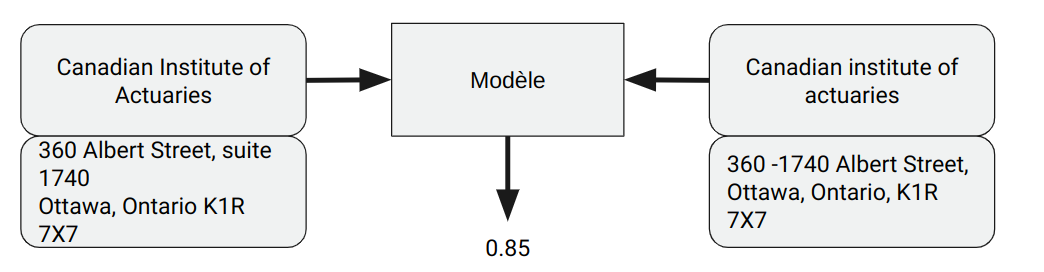
\includegraphics[width=0.9\linewidth]{img/sim}
		\end{figure}
		\link{https://corpus.ulaval.ca/server/api/core/bitstreams/c37706b1-c6e6-4878-8b3d-8a0874bba131/content}{Détection de doublons parmi des informations non structurées provenant de sources de données différentes}
	\end{frame}
	
	\begin{frame}{Similarité d'entité}
		\begin{figure}
			\centering
			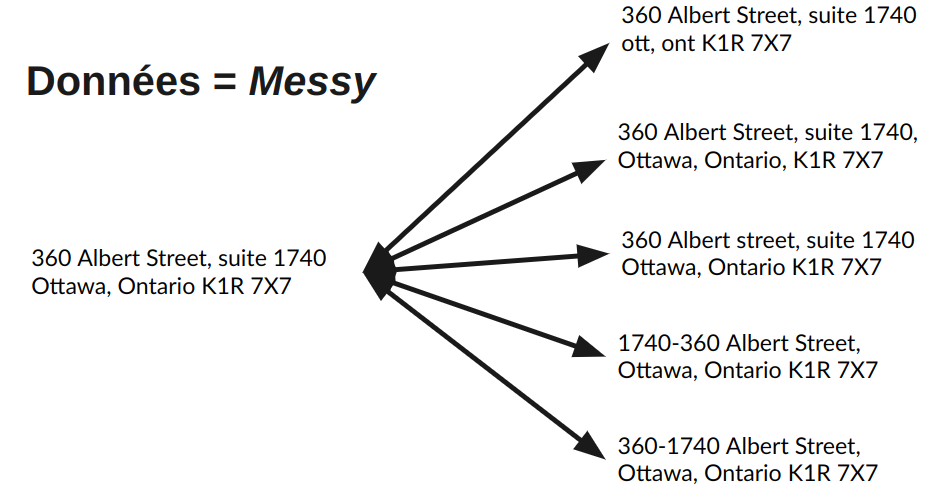
\includegraphics[width=0.7\linewidth]{img/messy}
		\end{figure}
	\end{frame}
	
	\begin{frame}{Similarité d'entité}
		\centering
		360 Albert Street, suite 1740$\arrowvert$ 360 Albert Street, Bureau 1740
	\end{frame}
	
	\begin{frame}{Similarité d'entité}
		\centering
		\begin{tabular}{cc|cc}
			\multicolumn{2}{c}{\textbf{Adresse \#1}} & \multicolumn{2}{c}{\textbf{Adresse \#2}}\\
			\toprule
			\textbf{Numéro civique} & 360  &\textbf{Numéro civique} & 360\\
			\textbf{Unité} & suite 1740 & \textbf{Unité} & bureau 1740 \\
			\textbf{Nom de la rue}  & Albert Street & \textbf{Nom de la rue}  & Albert Street\\
			\textbf{Orientation}    & $\emptyset$   & \textbf{Orientation}    & $\emptyset$  \\
			\textbf{Code postal}    & $\emptyset$ & \textbf{Code postal}    & $\emptyset$\\
		\end{tabular}
	\end{frame}
	
	\begin{frame}{Similarité d'entité}
		\begin{block}{Similarité de Jaccard}	
			\begin{equation*}
				\text{Jaccard}(\text{A, B}) =
				\begin{cases}
					0 & \text{si } |\text{A} \cap \text{B}| = 0 \text{ ou } |\text{A} \cup \text{B}| = 0\\
					\frac{|\text{A} \cap \text{B}|}{|\text{A} \cup \text{B}|} & \text{autrement}
				\end{cases}
			\end{equation*}
		\end{block}
		\begin{block}{Exemple}	
			\begin{center}
				Jaccard(Laval University, Montreal University)
				\bigskip\\ $\Downarrow$ \\ \bigskip
				$\frac{|\left\{\text{University}\right\}|}{|\left\{\text{University, Montreal, Laval}\right\}|} = \frac{1}{3} = \textbf{0,333}$
			\end{center}
		\end{block}
	\end{frame}
	
	\section{Plongements de sous-mots}
	\begin{frame}{Plongements de sous-mots}
		\uncover<1->{\textbf{Plongement de mot}: représentation vectorielle d'un mot}
		\begin{figure}
			\centering
			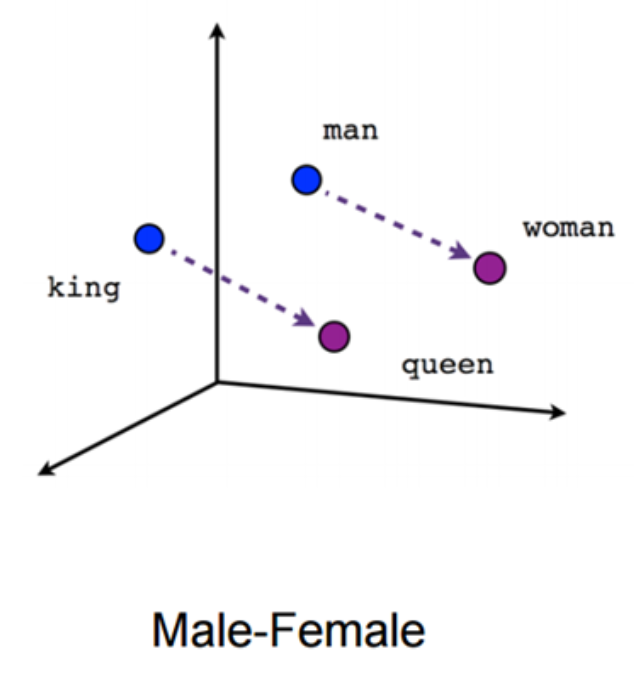
\includegraphics[width=0.3\linewidth]{img/wem}
		\end{figure}
		
		\uncover<2->{\textbf{\textit{Subword embedding}}: représentation d'une plus petite unité}
		\begin{itemize}
			\item<2-> Sous-chaîne de \textit{n-grams} (e.g: Le bi-gram de "H1A 1B1" est \{H1, 1A, A1, 1B, B1\})
		\end{itemize}
		
	\end{frame}
	
	\begin{frame}{Pourquoi?}
		Support multilingue (MultiBPEmb) et support pour mot hors vocabulaire (FastText).
	\end{frame}
	
	\section{Architecture}
	\begin{frame}{Modèles de plongements de mots}
		\begin{itemize}
			\item FastText
			\item MultiBPEmb
		\end{itemize}
	\end{frame}
	
	\begin{frame}{Modèle de segmentation}
		Nous utilisons un modèle Seq2Seq composé d'
		\begin{itemize}
			\item<2-> un encodeur LSTM unidirectionnel à une couche,
			\item<3-> un décodeur LSTM unidirectionnel à une couche,
			\item<4-> une couche linéaire entièrement connectée pour mapper la représentation dans la dimensionnalité de l'espace des étiquettes, et
			\item<5-> une fonction d'activation. 
		\end{itemize}
		
		\uncover<5->{Les états cachés du codeur et du décodeur sont tous deux de dimension $1024$.}
	\end{frame}
	
	\begin{frame}{Architecture}
		\begin{figure}[h!]
			\centering
			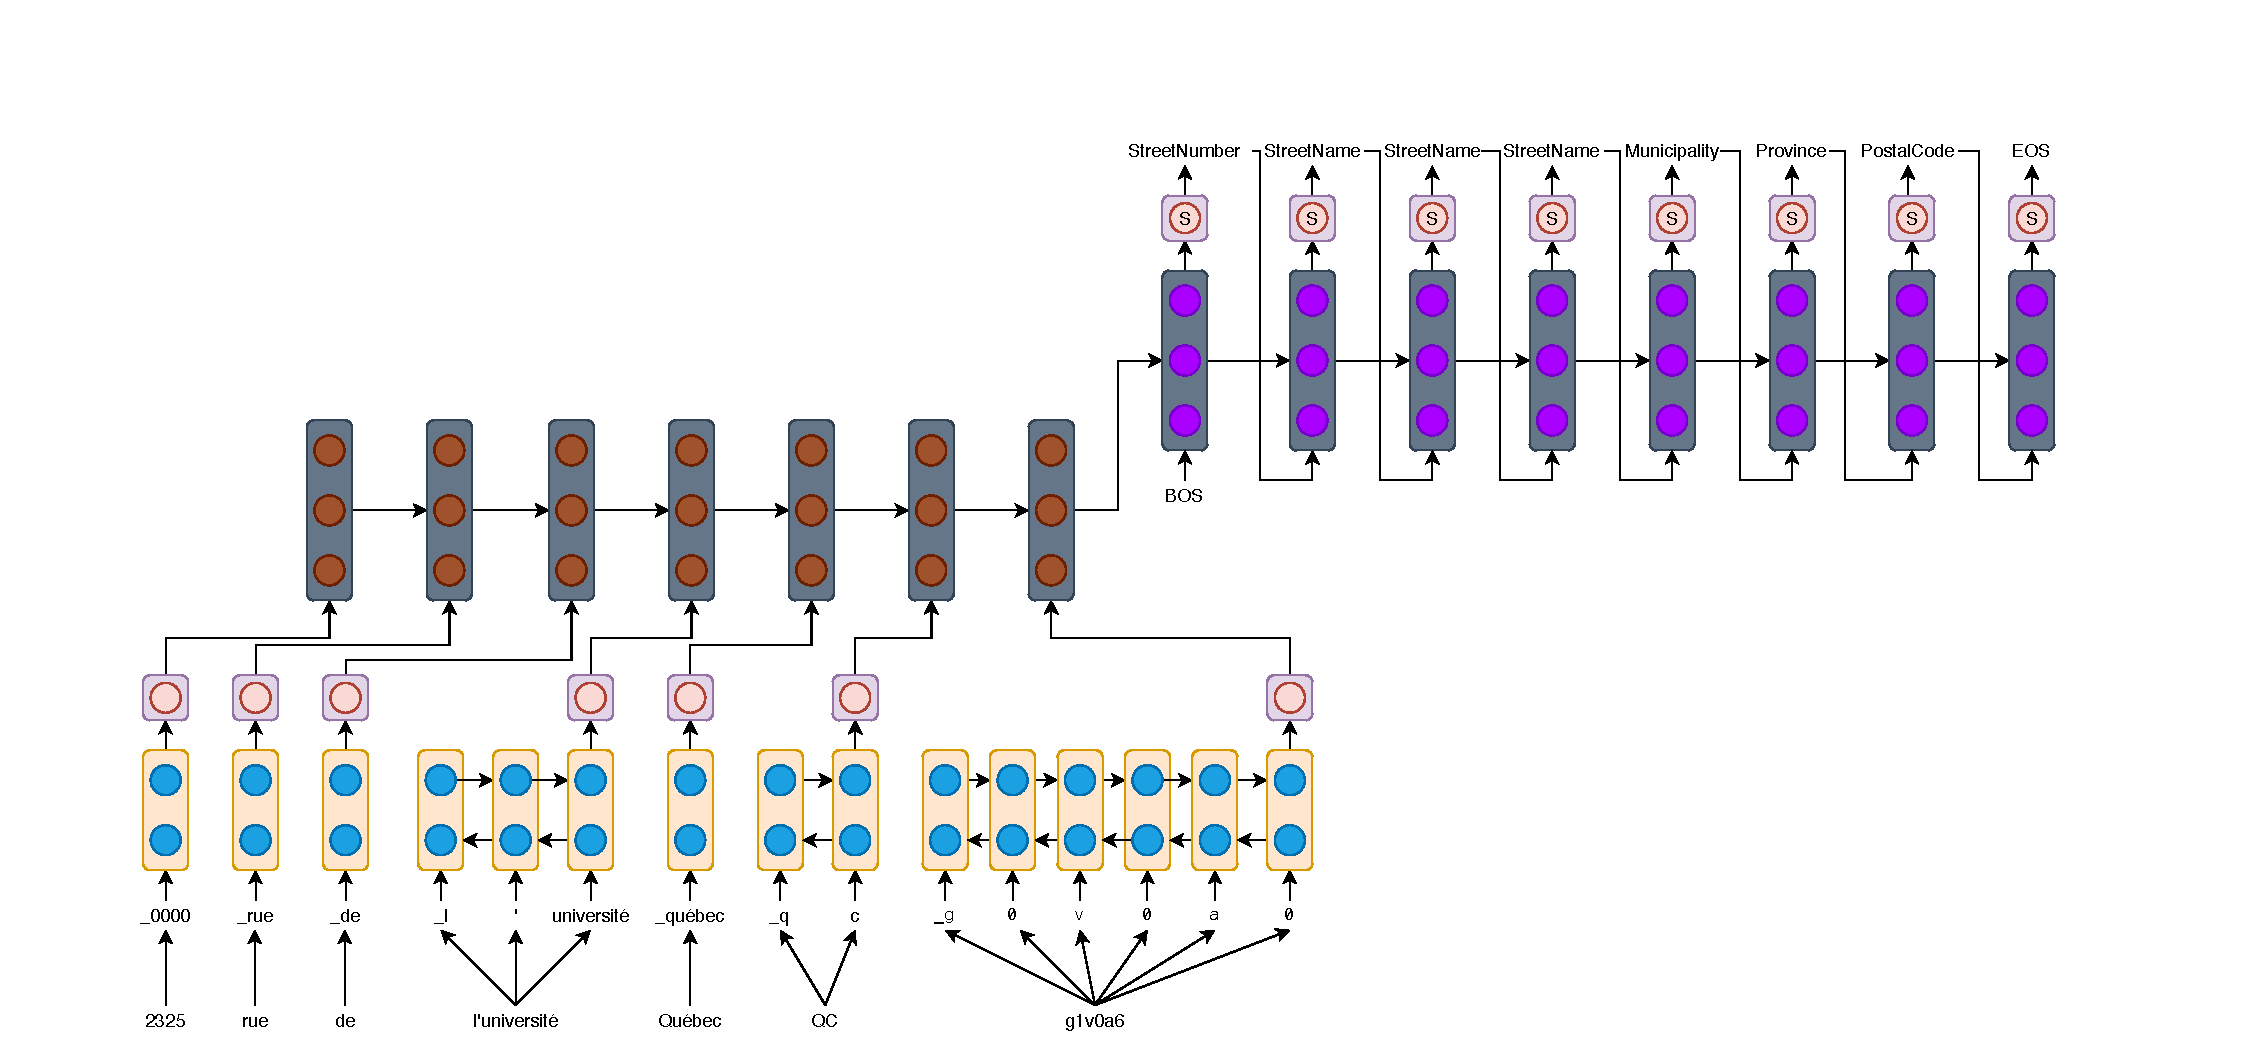
\includegraphics[width=1.1\textwidth,height=\textheight,keepaspectratio]{Network.pdf}
		\end{figure}
	\end{frame}
	
	\section{Entraînement}
	\begin{frame}{À propose de l'entraînement}
		\begin{itemize}
			\item Jeu de données public en ligne qui contient des millions d'adresses.
			\item $61$ pays sélectionner (avec un minimum de 100 adresses).
			\item 8 étiquettes: StreetNumber, StreetName, Unit, Municipality, Province, PostalCode, Orientation, et GeneralDelivery.
		\end{itemize}
	\end{frame}	
	
	\begin{frame}{Exemples d'adresses d'entraînement}
		\begin{figure}[h!]
			\centering
			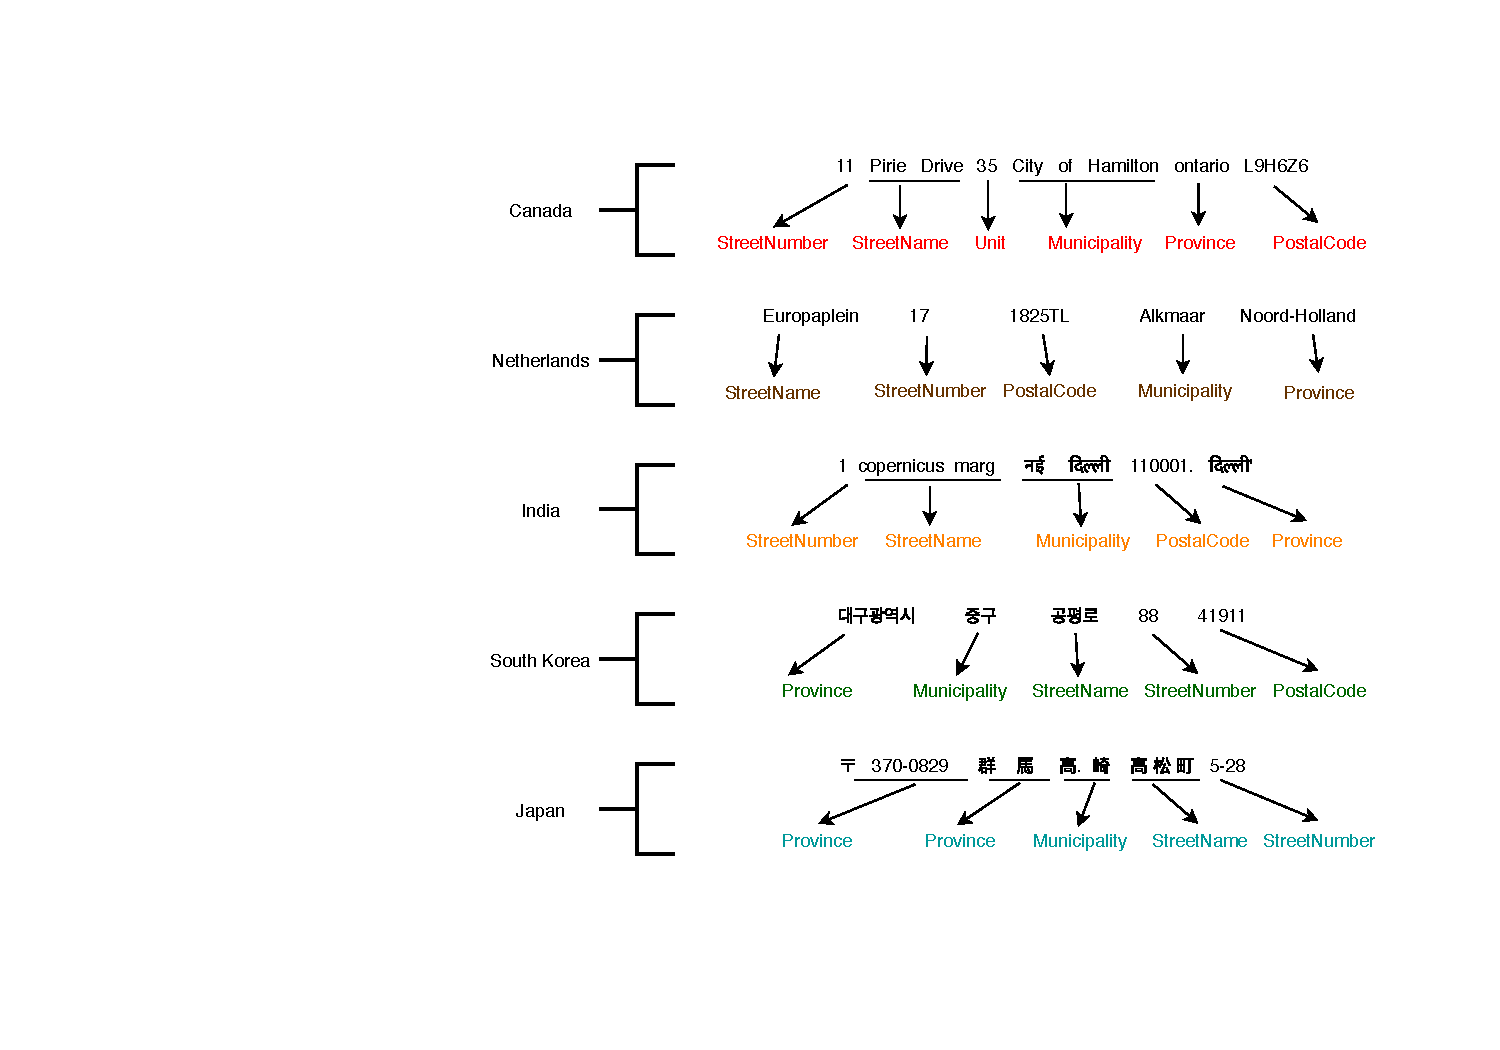
\includegraphics[width=0.8\textwidth,height=0.75\textheight,keepaspectratio]{Samples2.pdf}
		\end{figure}
	\end{frame}
	
	\begin{frame}{Performance}
		\resizebox{\textwidth}{!}{%
			\begin{tabular}{cccccc}
				\toprule
				Pays & \textbf{FastText} & \textbf{BPEmb} & Pays & \textbf{FastText} & \textbf{BPEmb}\\
				\midrule
				United States & $\mathbf{99.61 \pm 0.09}$ & $98.55 \pm 2.19$ & Poland & $\mathbf{99.69 \pm 0.07}$ & $99.19 \pm 1.39$\\
				Brazil & $\mathbf{99.40 \pm 0.10}$ & $98.54 \pm 1.68$ & Norway & $\mathbf{99.46 \pm 0.06}$ & $97.98 \pm 1.31$\\
				South Korea & $99.96 \pm 0.01$ & $\mathbf{99.99 \pm 0.02}$ & Austria & $\mathbf{99.28 \pm 0.03}$ & $98.28 \pm 1.56$\\
				Australia & $\mathbf{99.68 \pm 0.05}$ & $99.21 \pm 1.17$ & Finland & $\mathbf{99.77 \pm 0.03}$ & $99.72 \pm 0.30$\\
				Mexico & $\mathbf{99.60 \pm 0.06}$ & $98.55 \pm 2.22$ & Denmark & $\mathbf{99.71 \pm 0.07}$ & $99.20 \pm 1.38$\\
				Germany & $\mathbf{99.77 \pm 0.04}$ & $99.23 \pm 1.30$ & Czechia & $\mathbf{99.57 \pm 0.09}$ & $98.77 \pm 2.22$\\
				Spain & $\mathbf{99.75 \pm 0.05}$ & $98.65 \pm 2.36$ & Italy & $\mathbf{99.73 \pm 0.05}$ & $98.91 \pm 1.76$\\
				Netherlands & $\mathbf{99.61 \pm 0.07}$ & $99.26 \pm 1.23$ & France & $\mathbf{99.66 \pm 0.08}$ & $98.65 \pm 2.00$\\
				Canada & $\mathbf{99.79 \pm 0.05}$ & $99.19 \pm 1.33$ & United Kingdom & $\mathbf{99.61 \pm 0.10}$ & $98.66 \pm 2.11$\\
				Switzerland & $\mathbf{99.53 \pm 0.09}$ & $99.49 \pm 0.53$ & Russia & $\mathbf{99.03 \pm 0.24}$ & $97.52 \pm 4.23$\\
				\bottomrule
			\end{tabular}%
		}
	\end{frame}

	\begin{frame}{Performance}
		\begin{itemize}
			\item Évaluation en zero-shot.
			\item Modèle avec attention.
			\item Modèle avec entraînement par adaptation de domaine (ADAN).
			\item Tests de significativité.
		\end{itemize}
	\end{frame}
	
	\section{Conclusion}
	\begin{frame}{Conclusion}
		Deepparse permet
		\begin{itemize}
			\item de séparer les composantes d'une adresse en plusieurs langues, notament en français et en anglais,
			\item d'ajuster nos modèles sur son jeu de données, et
			\item de changer les étiquettes.
		\end{itemize}		
		Pour en savoir plus, lire nos deux articles \url{https://arxiv.org/abs/2006.16152} et \url{https://arxiv.org/abs/2112.04008}
	\end{frame}
	
	\begin{frame}{Questions}
		\centering
		\fontsize{100}{100}\faQuestion
	\end{frame}
	
	
\end{document}